\documentclass[tikz,border=8pt]{standalone}
% Shared look for every TikZ diagram. Load with \input{../../tools/tikz-style.tex}
\usepackage[sfdefault]{roboto}
\usetikzlibrary{arrows.meta, positioning, shapes.geometric, calc, fit, backgrounds}
\definecolor{cblue}{HTML}{4C78A8}
\definecolor{corange}{HTML}{F58518}
\definecolor{cgreen}{HTML}{54A24B}
\definecolor{cred}{HTML}{E45756}
\definecolor{cpurple}{HTML}{B279A2}
\definecolor{cgrey}{HTML}{6B6B6B}
\tikzset{
  every picture/.style={font=\sffamily, line width=1.2pt},
  box/.style={draw=#1, fill=#1!12, rounded corners=4pt, align=center, inner sep=7pt, minimum height=1.1cm},
  box/.default=cgrey,
  arrow/.style={-{Stealth[length=3mm]}, draw=cgrey, line width=1.4pt},
  title/.style={font=\sffamily\bfseries\Large},
  note/.style={font=\sffamily\small, text=cgrey, align=center},
}
\AtBeginDocument{\hyphenpenalty=10000 \exhyphenpenalty=10000}

\usepackage{amssymb}
% The task of the Note in the room of RO-009: the cup stands on the table; carry it to the door. Three places:
% start (the robot at (2, 1)), table (beside the table, 2.75, 1.75) and door (just inside the doorway, 3.75, 3.75).
\begin{document}
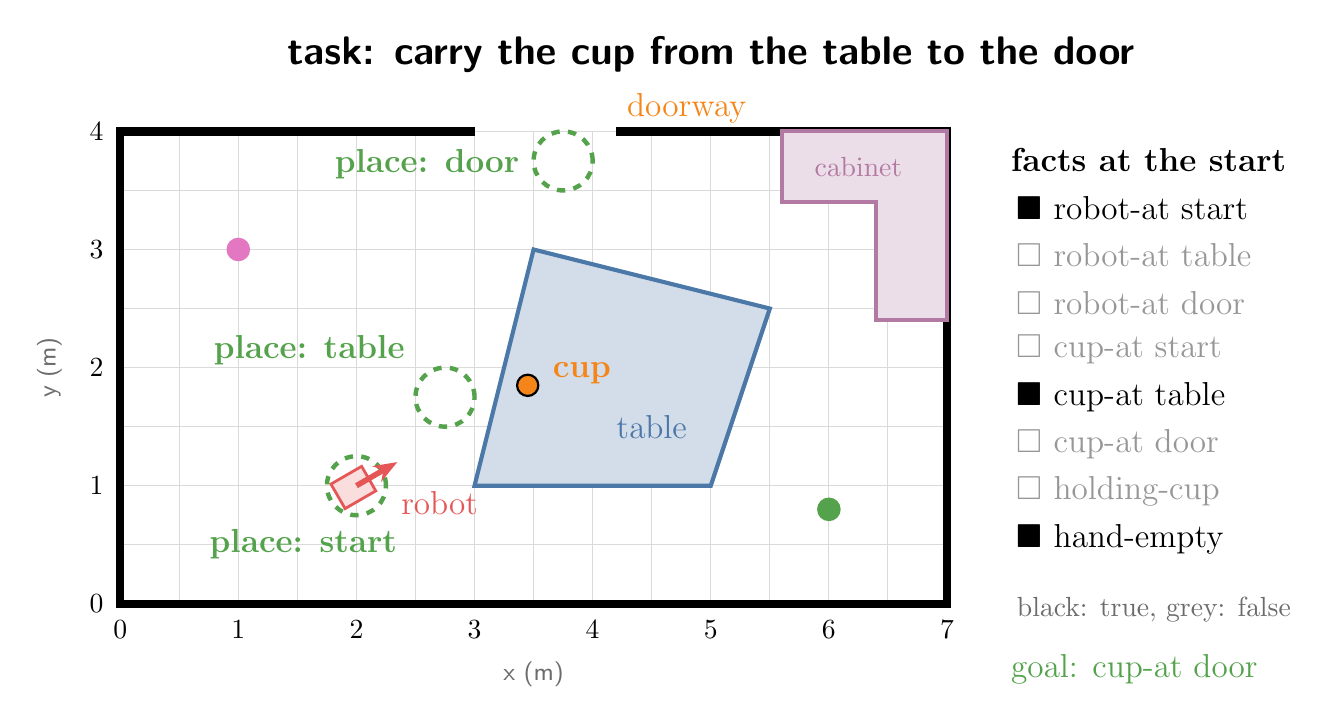
\begin{tikzpicture}[scale=1.5, every node/.append style={font=\large}]
  \definecolor{cpink}{HTML}{E377C2}
  \draw[cgrey!25, line width=0.4pt] (0,0) grid[step=0.5] (7,4);
  \draw[black, line width=3pt] (3.0,4) -- (0,4) -- (0,0) -- (7,0) -- (7,4) -- (4.2,4);
  \filldraw[cblue!25, draw=cblue, line width=1.5pt] (3,1) -- (5,1) -- (5.5,2.5) -- (3.5,3) -- cycle;
  \node[cblue] at (4.5,1.5) {table};
  \filldraw[cpurple!25, draw=cpurple, line width=1.5pt] (5.6,4) -- (5.6,3.4) -- (6.4,3.4) -- (6.4,2.4) -- (7,2.4) -- (7,4) -- cycle;
  \node[cpurple, font=\normalsize] at (6.25,3.7) {cabinet};
  \fill[cpink] (1,3) circle (0.1);
  \fill[cgreen] (6,0.8) circle (0.1);
  % the cup on the table
  \filldraw[corange, draw=black, line width=0.8pt] (3.45,1.85) circle (0.09);
  \node[corange, right=3pt, font=\bfseries\large] at (3.5,1.95) {cup};
  % the three places
  \foreach \x/\y/\n/\p in {2.0/1.0/start/below left, 2.75/1.75/table/above left, 3.75/3.75/door/left} {
    \draw[cgreen, dashed, line width=1.6pt] (\x,\y) circle (0.25);
  }
  \node[cgreen, font=\bfseries\large, anchor=north] at (1.55,0.72) {place: start};
  \node[cgreen, font=\bfseries\large, anchor=east] at (2.5,2.15) {place: table};
  \node[cgreen, font=\bfseries\large, anchor=east] at (3.47,3.72) {place: door};
  \node[corange, above right] at (4.2,3.98) {doorway};
  % the robot at the start
  \begin{scope}[shift={(2,1)}, rotate=30]
    \draw[cred, fill=cred!20, line width=1pt] (-0.18,-0.12) rectangle (0.12,0.12);
    \draw[-{Stealth[length=3mm]}, cred, line width=2pt] (0,0) -- (0.4,0);
  \end{scope}
  \node[cred, right=8pt] at (2.1,0.85) {robot};
  % the task
  \node[title] at (5.0,4.65) {task: carry the cup from the table to the door};
  % the facts at the start
  \node[anchor=north west, font=\bfseries\large] at (7.45,3.95) {facts at the start};
  \foreach \i/\f/\v in {1/robot-at start/1, 2/robot-at table/0, 3/robot-at door/0, 4/cup-at start/0,
      5/cup-at table/1, 6/cup-at door/0, 7/holding-cup/0, 8/hand-empty/1} {
    \ifnum\v=1
      \node[anchor=west, font=\large] at (7.5,3.75-0.4*\i) {$\blacksquare$ \f};
    \else
      \node[anchor=west, font=\large, text=cgrey!70] at (7.5,3.75-0.4*\i) {$\square$ \f};
    \fi
  }
  \node[anchor=west, note, font=\normalsize, align=left] at (7.5,-0.05) {black: true, grey: false};
  \node[anchor=west, font=\large, text=cgreen] at (7.45,-0.55) {goal: cup-at door};
  \foreach \t in {0,...,7} \node[below, font=\normalsize] at (\t,-0.05) {\t};
  \foreach \t in {0,...,4} \node[left, font=\normalsize] at (-0.05,\t) {\t};
  \node[note] at (3.5,-0.6) {x (m)}; \node[note, rotate=90] at (-0.6,2) {y (m)};
\end{tikzpicture}
\end{document}
